\documentclass{standalone}

\usepackage[english]{babel} % English language/hyphenation
\usepackage{graphicx} % Required for including pictures
\usepackage{tikz} % Required for drawing custom shapes
\usetikzlibrary{arrows}
\usetikzlibrary{shapes.misc}
\usetikzlibrary{decorations.pathreplacing}

\begin{document}
	\def\glider#1#2#3{
		\begin{scope}[shift={#1}, rotate=#2, scale=#3]
			\fill[black](0,0) -- (1,0) -- (1,1) -- (0,1) -- cycle;
			\fill[black](8/7+0,0) -- (8/7+1,0) -- (8/7+1,1) -- (8/7+0,1) -- cycle;
			\fill[black](16/7+0,0) -- (16/7+1,0) -- (16/7+1,1) -- (16/7+0,1) -- cycle;
			\fill[black](16/7+0,8/7+0) -- (16/7+1,8/7+0) -- (16/7+1,8/7+1) -- (16/7+0,8/7+1) -- cycle;
			\fill[black](8/7+0,16/7+0) -- (8/7+1,16/7+0) -- (8/7+1,16/7+1) -- (8/7+0,16/7+1) -- cycle;
		\end{scope}
	}
	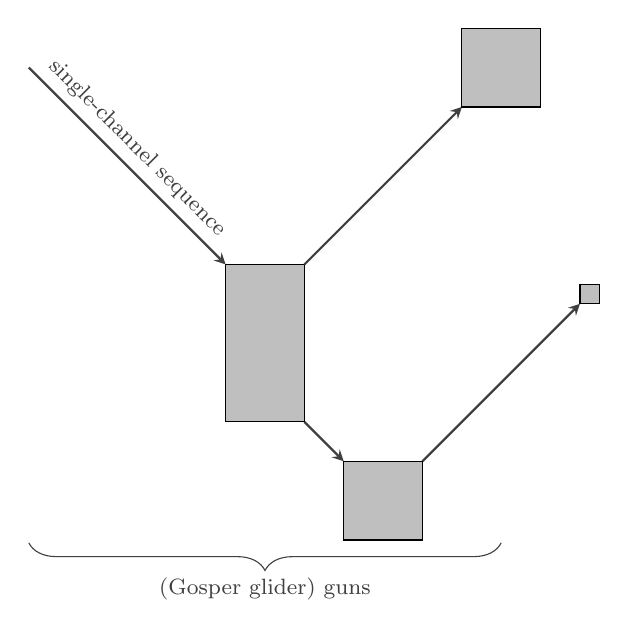
\begin{tikzpicture}%
		% SOURCE glider stream from top-left
		\glider{(-0.25,6)}{0}{0.08};
		\draw[thick,color=darkgray,-stealth] (0,6) -- (2.5,3.5);
		\draw[darkgray]	(1.2,4.8) node [anchor=south,rotate=-45]{\footnotesize single-channel sequence};
		
		% SCORBIE SPLITTER
		\filldraw[color=black,fill=gray!50] (2.5,3.5) -- (3.5,3.5) -- (3.5,1.5) -- (2.5,1.5) -- cycle;
		
		% Output of scorbie splitter
		\draw[thick,color=darkgray,-stealth] (3.5,1.5) -- (4,1);
		\draw[thick,color=darkgray,-stealth] (3.5,3.5) -- (5.5,5.5);
		\draw[thick,color=darkgray,-stealth] (5,1) -- (7,3);
		
		% SNARKS
		\filldraw[color=black,fill=gray!50] (4,1) -- (5,1) -- (5,0) -- (4,0) -- cycle;
		\filldraw[color=black,fill=gray!50] (5.5,5.5) -- (6.5,5.5) -- (6.5,6.5) -- (5.5,6.5) -- cycle;
		
		% TARGET BLOCK, turned into CORDERSHIP
		\filldraw[color=black,fill=gray!50] (7,3) -- (7,3.25) -- (7.25,3.25) -- (7.25,3) -- cycle;
		
		
		\draw[darkgray,decorate,decoration={brace,amplitude=10pt,mirror},yshift=-1pt]
		(0,0) --node [anchor=north,yshift=-9pt]{\footnotesize (Gosper glider) guns} (6,0);
	\end{tikzpicture}
\end{document}